% ----------------------------------------------------------------------------------------------------- %
% Manual da Classe UFTeX
% 
% Versão 2.1:   Março 2018
%
% Criado por:   Tiago da Silva Almeida
% Revisado por: Tiago da Silva Almeida
%               Rafael Lima de Carvalho
%               Ary Henrique Morais de Oliveira
%
% https://almeidatiago.github.io/uftex/
% ----------------------------------------------------------------------------------------------------- %

\documentclass[tcc2]{uftex}
% ---- Esse comando cria o nome uftex estilizado
\newcommand\uftex{UF\TeX}

\usepackage{lipsum}
\usepackage{tikz}
\usepackage[siunitx]{circuitikz}
\usepackage{pgfplots}
\usepackage{pgfplotstable}

\pgfplotsset{compat=1.18}
\usetikzlibrary{arrows}

\usepackage[alf,abnt-emphasize=bf]{abntex2cite}
\renewcommand{\backrefpagesname}{}
\renewcommand{\backref}{}
\renewcommand*{\backrefalt}[4]{}
% ----  Esse comandos são necessário no pré-ambulo para a impressão da lista de lista abreviatuas e de símbolos
\makelosymbols
\makeloabbreviations
% ---- Início do documento
\begin{document}
  % ---- Descrição do título do trabalho 
  \title{Análise Empírica de Algoritmos de Ordenação}
  % ---- Nome do autor ou autores do trabalho
  \author{Caio Santos Silva, Gustavo Gonzaga dos Santos e Thiago Gonzaga dos Santos}{}

  % ---- Nome do orientador do trabalho. O último campo representa o título do professor
  \advisor{Prof.}{Tiago}{da Silva Almeida}{Me.}

  \examiner{Prof.}{Dr.}{Nome do Primeiro Examinador Sobrenome}
  \examiner{Profa.}{Dra.}{Nome do Segundo Examinador Sobrenome}
  \examiner{Profa.}{Ma.}{Nome do Terceiro Examinador Sobrenome}
  % ---- Departamento representa o curso ao qual o trabalho está sendo apresentado. Descrito por meio de duas iniciais do curso
  \department{CC}
  % ---- Data da apresentação do trabalho
  \date{25}{03}{2024}
  % ---- Palavras-chaves em português do trabalho
  \keyword{Algoritmos de Ordenação}
  \keyword{Complexidade de Tempo}
  \keyword{Análise Empírica}
  \keyword{Comparações}
  \keyword{Eficiência Computacional}
  % ---- Palavras-chaves em inglês do trabalho
  \foreignkeyword{Sorting Algorithms}
  \foreignkeyword{Time Complexity}
  \foreignkeyword{Empirical Analysis}
  \foreignkeyword{Comparisons}
  \foreignkeyword{Computational Efficiency}
  
  % ---- Comando responsável por criar a capa do trabalho, logo em seguida está o comando que insere a folha de rosto conforme a configuração exigida
 \maketitle

% Esse comando Insere a Folha de Rosto
 % \frontmatter

  \begin{abstract}
  Este trabalho realiza uma análise empírica de seis algoritmos de ordenação: Bubble Sort, Selection Sort, Insertion Sort, Merge Sort, Quick Sort e Heap Sort. Foram implementados e testados esses algoritmos em listas de diferentes tamanhos (1.000, 10.000, 50.000 e 100.000 elementos), com distribuições ordenadas, inversamente ordenadas e aleatórias. A análise focou na medição do tempo de execução, número de comparações e número de trocas realizadas por cada algoritmo. Os resultados mostraram diferenças significativas de desempenho, destacando as vantagens de algoritmos como o Merge Sort e o Quick Sort em listas grandes e desordenadas, enquanto algoritmos simples como o Insertion Sort mostraram eficiência em listas pequenas ou parcialmente ordenadas. Com base nesses resultados, são discutadas as melhores escolhas de algoritmos dependendo do cenário de aplicação.
  \end{abstract}

  \begin{foreignabstract}
  This paper conducts an empirical analysis of six sorting algorithms: Bubble Sort, Selection Sort, Insertion Sort, Merge Sort, Quick Sort, and Heap Sort. These algorithms were implemented and tested on lists of varying sizes (1,000, 10,000, 50,000, and 100,000 elements) with ordered, reverse ordered, and random distributions. The analysis focused on measuring execution time, the number of comparisons, and the number of swaps performed by each algorithm. The results demonstrated significant performance differences, highlighting the advantages of algorithms such as Merge Sort and Quick Sort for large, unsorted lists, while simpler algorithms like Insertion Sort showed efficiency in smaller or partially ordered lists. Based on these findings, recommendations are made for the best algorithm choices depending on specific sorting scenarios.
  \end{foreignabstract}
  \printlosymbols  
  \printloabbreviations
  % ---- Cria a lista de figuras. OPCIONAL
  \listoffigures
  % ---- Cria a lista de tabelas. OPCIONAL
  \listoftables 
  % ---- Cria o sumário. OBRIGATÓRIO
  \tableofcontents % sumário
% --- Marca o inicio dos elementos textuais. Capítulos.
\mainmatter
% ---- Defino o espaçamento de um e meio centímetros
\onehalfspacing
% ----------------------------------------------------------------------------------------------------- %
% Capítulos do trabalho
% ----------------------------------------------------------------------------------------------------- %
\ChapterStart{first}{First chapter}

\chapter{Introdução}
\section{Importância da ordenação de dados}
A ordenação é amplamente considerada um dos problemas mais fundamentais no estudo de algoritmos. Isso se deve a diversos fatores. Em algumas aplicações, a ordenação é uma necessidade intrínseca; por exemplo, bancos precisam organizar cheques por número para preparar extratos de clientes. Além disso, a ordenação é frequentemente usada como sub-rotina em outros algoritmos. Um exemplo comum é em programas que renderizam objetos gráficos, onde é necessário ordenar os objetos de acordo com a relação de profundidade para desenhá-los corretamente, do fundo para a frente. \cite{2022:Thomas}



\section{Objetivo}
Este trabalho tem como objetivo comparar seis algoritmos de ordenação: Bubble Sort, Selection Sort, Insertion Sort, Merge Sort, Quick Sort e Heap Sort. A análise será realizada tanto do ponto de vista teórico quanto empírico, medindo o tempo de execução, número de comparações e trocas em diferentes listas de tamanhos e distribuições.


\chapter{Revisão Teórica}

Na ciência da computação, algoritmos de ordenação são essenciais para organizar dados de maneira eficiente. A escolha do algoritmo de ordenação adequado pode ter um impacto significativo no desempenho de programas, especialmente em grandes volumes de dados. Cada algoritmo tem suas próprias características, como a complexidade de tempo, o consumo de memória e a estabilidade, que o tornam mais ou menos adequado para diferentes tipos de problemas. Nesta seção, são discutidos seis algoritmos de ordenação: Bubble Sort, Selection Sort, Insertion Sort, Merge Sort, Quick Sort e Heap Sort. A seguir, é apresentada a descrição teórica de cada um deles, com ênfase nas propriedades que influenciam sua eficiência em diferentes contextos.

\section{Bubble Sort}
O Bubble Sort é um algoritmo simples que funciona repetidamente comparando pares adjacentes e trocando-os se estiverem na ordem errada. Sua complexidade é \(O(n^2)\) no pior caso e \(O(n)\) no melhor caso (quando a lista já está ordenada).

\begin{itemize}
    \item Complexidade: \(O(n^2)\).
    \item In-place: Sim.
    \item Estabilidade: Sim.
\end{itemize}

\section{Selection Sort}
O Selection Sort divide o vetor em duas partes: a parte ordenada e a parte não ordenada. A cada iteração, o menor elemento da parte não ordenada é selecionado e colocado na posição correta. Sua complexidade também é \(O(n^2)\).

\begin{itemize}
    \item Complexidade: \(O(n^2)\).
    \item In-place: Sim.
    \item Estabilidade: Não.
\end{itemize}

\section{Insertion Sort}
O Insertion Sort constrói uma lista ordenada um elemento de cada vez. Ele tem complexidade \(O(n^2)\) no pior caso, mas pode ser \(O(n)\) se a lista já estiver quase ordenada.

\begin{itemize}
    \item Complexidade: \(O(n^2)\).
    \item In-place: Sim.
    \item Estabilidade: Sim.
\end{itemize}


\section{Merge Sort}
O Merge Sort utiliza o método de divisão e conquista para ordenar os elementos. Ele divide a lista em sublistas até que cada sublista tenha um único elemento e, em seguida, as combina. Sua complexidade é \(O(n \log n)\).

\begin{itemize}
    \item Complexidade: \(O(n \log n)\).
    \item In-place: Não.
    \item Estabilidade: Sim.
\end{itemize}

\section{Quick Sort}
O Quick Sort também utiliza o método de divisão e conquista. Ele seleciona um "pivô"  e particiona os outros elementos em duas sublistas de acordo com se eles são menores ou maiores que o pivô. Sua complexidade média é \(O(n \log n)\).

\begin{itemize}
    \item Complexidade: \(O(n \log n)\) no melhor caso, \(O(n²)\) no pior caso.
    \item In-place: Sim.
    \item Estabilidade: Não.
\end{itemize}

\section{Heap Sort}
O Heap Sort transforma a lista em uma estrutura de heap e então extrai os elementos da heap para formar a lista ordenada. Sua complexidade é \(O(n \log n)\).

\begin{itemize}
    \item Complexidade: \(O(n \log n)\).
    \item In-place: Sim.
    \item Estabilidade: Não.
\end{itemize}

\chapter{Metodologia}

%\begin{lstlisting}[language=python]
%def bubble_sort(arr):
%    n = len(arr)
%    for i in range(n):
%        for j in range(0, n-i-1):
%            if arr[j] > arr[j+1]:
%                arr[j], arr[j+1] = arr[j+1], arr[j]
%
%\end{lstlisting}

Para a realização dos testes empíricos, a metodologia adotada inclui a implementação dos algoritmos de ordenação, a geração de listas de diferentes tamanhos e distribuições, e a medição do desempenho dos algoritmos. A seguir, são apresentados os detalhes de cada etapa.

\section{Ambiente de Teste}

\begin{itemize}
    \item Hardware: AMD Ryzen 7, 64GB memória RAM, Windows 11 64 bits.
    \item Software: Linguagem de programação Python e bibliotecas .
\end{itemize}

\section{Implementação}
Para a implementação dos algoritmos de ordenação, foram desenvolvidos dois códigos em Python. O primeiro código é responsável pela geração das listas, enquanto o segundo realiza a ordenação dessas listas utilizando os diferentes algoritmos de ordenação. Além disso, o segundo código calcula o tempo de execução e o número de comparações realizadas durante o processo de ordenação.


As listas para os testes foram geradas com diferentes distribuições (ordenadas, inversamente ordenadas e aleatórias). O código abaixo ilustra o processo de geração das listas e como são salvas em arquivos:

\begin{lstlisting}[language=python]
import random

def gerar_listas(tamanho):
    lista_ordenada = list(range(1, tamanho + 1))
    lista_inversa = list(range(tamanho, 0, -1))
    lista_aleatoria = lista_ordenada[:]
    random.shuffle(lista_aleatoria)
    return lista_ordenada, lista_inversa, lista_aleatoria

def salvar_listas(tamanho):
    lista_ordenada, lista_inversa, lista_aleatoria = gerar_listas(tamanho)
    nome_arquivo = f'lista_{tamanho}.txt'
    with open(nome_arquivo, 'w') as f:
        f.write(', '.join(map(str, lista_ordenada)) + '\n')
        f.write(', '.join(map(str, lista_inversa)) + '\n')
        f.write(', '.join(map(str, lista_aleatoria)) + '\n')

for tamanho in [1000, 10000, 50000, 100000]:
    salvar_listas(tamanho)
    print(f"Arquivo 'lista_{tamanho}.txt' gerado com sucesso!")

\end{lstlisting}

Esse código gera três tipos de listas para cada tamanho de dados testado (1.000, 10.000, 50.000 e 100.000 elementos):
\begin{itemize}
    \item Lista Ordenada: Elementos em ordem crescente.
    \item Lista Inversamente Ordenada: Elementos em ordem decrescente.
    \item Lista Aleatória: Elementos dispostos em uma ordem aleatória.
\end{itemize}
    
   

Cada lista foi salva em um arquivo .txt, contendo as três versões (ordenada, inversa e aleatória) para cada tamanho. Esses arquivos serviram de entrada para os algoritmos de ordenação.

Foram implementados seis algoritmos de ordenação: Bubble Sort, Selection Sort, Insertion Sort, Merge Sort, Quick Sort e Heap Sort. A implementação de cada algoritmo contabiliza o número de comparações e trocas realizadas, além de medir o tempo de execução. O código para execução dos algoritmos é descrito abaixo.
\begin{itemize}


\item{Bubble Sort}

\begin{lstlisting}[language=python]
def bubble_sort(arr):
    comparacoes, trocas = 0, 0
    for i in range(len(arr)):
        for j in range(0, len(arr) - i - 1):
            comparacoes += 1
            if arr[j] > arr[j + 1]:
                arr[j], arr[j + 1] = arr[j + 1], arr[j]
                trocas += 1
    return comparacoes, trocas
\end{lstlisting}

\item{Selection Sort}


\begin{lstlisting}[language=python]
def selection_sort(arr):
    comparacoes, trocas = 0, 0
    for i in range(len(arr)):
        min_idx = i
        for j in range(i + 1, len(arr)):
            comparacoes += 1
            if arr[j] < arr[min_idx]:
                min_idx = j
        if min_idx != i:
            arr[i], arr[min_idx] = arr[min_idx], arr[i]
            trocas += 1
    return comparacoes, trocas

\end{lstlisting}

\item{Insertion Sort}


\begin{lstlisting}[language=python]
def insertion_sort(arr):
    comparacoes, trocas = 0, 0
    for i in range(1, len(arr)):
        key = arr[i]
        j = i - 1
        comparacoes += 1
        while j >= 0 and key < arr[j]:
            arr[j + 1] = arr[j]
            trocas += 1
            j -= 1
            comparacoes += 1
        arr[j + 1] = key
    return comparacoes, trocas

\end{lstlisting}


\item{Merge Sort}

\begin{lstlisting}[language=python]
def merge_sort(arr):
    comparacoes = [0]
    def merge(arr, l, m, r):
        L = arr[l:m + 1]
        R = arr[m + 1:r + 1]
        i = j = k = 0
        while i < len(L) and j < len(R):
            comparacoes[0] += 1
            if L[i] <= R[j]:
                arr[k] = L[i]
                i += 1
            else:
                arr[k] = R[j]
                j += 1
            k += 1
        while i < len(L):
            arr[k] = L[i]
            i += 1
            k += 1
        while j < len(R):
            arr[k] = R[j]
            j += 1
            k += 1

    def sort(arr, l, r):
        if l < r:
            m = (l + r) // 2
            sort(arr, l, m)
            sort(arr, m + 1, r)
            merge(arr, l, m, r)
    
    sort(arr, 0, len(arr) - 1)
    return comparacoes[0], 0


\end{lstlisting}

\item{Quick Sort}


\begin{lstlisting}[language=python]
def quick_sort(arr):
    comparacoes = [0]
    def partition(arr, low, high):
        pivot = arr[high]
        i = low - 1
        for j in range(low, high):
            comparacoes[0] += 1
            if arr[j] < pivot:
                i += 1
                arr[i], arr[j] = arr[j], arr[i]
        arr[i + 1], arr[high] = arr[high], arr[i + 1]
        return i + 1

    def sort(arr, low, high):
        if low < high:
            pi = partition(arr, low, high)
            sort(arr, low, pi - 1)
            sort(arr, pi + 1, high)
    
    sort(arr, 0, len(arr) - 1)
    return comparacoes[0], 0

\end{lstlisting}

\item{Heap Sort}


\begin{lstlisting}[language=python]
def heap_sort(arr):
    comparacoes = [0]
    def heapify(arr, n, i):
        largest = i
        left = 2 * i + 1
        right = 2 * i + 2
        if left < n and arr[left] > arr[largest]:
            largest = left
        if right < n and arr[right] > arr[largest]:
            largest = right
        if largest != i:
            arr[i], arr[largest] = arr[largest], arr[i]
            heapify(arr, n, largest)

    n = len(arr)
    for i in range(n // 2 - 1, -1, -1):
        heapify(arr, n, i)
    for i in range(n - 1, 0, -1):
        arr[i], arr[0] = arr[0], arr[i]
        heapify(arr, i, 0)

    return comparacoes[0], 0

\end{lstlisting}
\end{itemize}

\section{Procedimento para Medir o Tempo de Execução, Comparações e Trocas}
Os dados foram gerados utilizando a função gerar\_listas(tamanho), que cria três tipos de listas para cada tamanho: ordenada, inversamente ordenada e aleatória. Os tamanhos de listas considerados foram 1.000, 10.000, 50.000 e 100.000 elementos.

Os algoritmos de ordenação foram executados em cópias dessas listas. O tempo de execução foi calculado com a função time.time() antes e depois da execução de cada algoritmo, e os valores foram multiplicados por mil para serem apresentados em milissegundos. Além disso, variáveis específicas em cada algoritmo foram usadas para rastrear o número de comparações (interações que comparam dois elementos) e trocas (operações de troca de posições entre elementos).

Os resultados obtidos foram organizados e analisados de maneira comparativa para cada algoritmo em relação ao tamanho da lista e à sua distribuição.

\chapter{Resultados}

Nesta seção, serão apresentados os resultados obtidos nos testes de desempenho dos algoritmos de ordenação. Os algoritmos foram executados em listas de diferentes tamanhos (1.000, 10.000, 50.000 e 100.000 elementos), com três tipos de organização: listas ordenadas, inversamente ordenadas e aleatórias. Os tempos de execução, número de comparações e número de trocas foram medidos para cada caso.

\section{Apresentação dos Resultados}
Os testes foram realizados em três tipos de listas: ordenadas, inversamente ordenadas e aleatórias. Abaixo, é apresentada uma síntese dos resultados obtidos para listas de 1.000, 10.000, 50.000 e 100.000 elementos. As tabelas abaixo apresentam os tempos de execução (em milissegundos), o número de comparações e o número de trocas para cada algoritmo.


\begin{table}[h]
\centering
\caption{Resultados para Lista de 1.000 Elementos}
\begin{tabular}{|l|l|l|l|l|}
\hline
\textbf{Algoritmo}   & \textbf{Tipo de Lista}       & \textbf{Tempo (ms)} & \textbf{Comparações} & \textbf{Trocas} \\ \hline
Bubble Sort          & Ordenada                     & 42.006              & 499.500              & 0              \\ \hline
Bubble Sort          & Inversamente Ordenada        & 79.014              & 499.500              & 499.500        \\ \hline
Bubble Sort          & Aleatória                    & 54.010              & 499.500              & 248.718        \\ \hline
Selection Sort       & Ordenada                     & 26.006              & 499.500              & 0              \\ \hline
Selection Sort       & Inversamente Ordenada        & 33.008              & 499.500              & 500            \\ \hline
Selection Sort       & Aleatória                    & 26.013              & 499.500              & 994            \\ \hline
Insertion Sort       & Ordenada                     & 0.000               & 999                  & 0              \\ \hline
Insertion Sort       & Inversamente Ordenada        & 71.015              & 500.499              & 499.500        \\ \hline
Insertion Sort       & Aleatória                    & 29.014              & 249.717              & 248.718        \\ \hline
Merge Sort           & Ordenada                     & 1.999               & 5.044                & 0              \\ \hline
Merge Sort           & Inversamente Ordenada        & 2.996               & 4.932                & 0              \\ \hline
Merge Sort           & Aleatória                    & 2.007               & 8.708                & 0              \\ \hline
Quick Sort           & Ordenada                     & 89.029              & 499.500              & 500.499        \\ \hline
Quick Sort           & Inversamente Ordenada        & 75.017              & 499.500              & 250.499        \\ \hline
Quick Sort           & Aleatória                    & 2.001               & 11.504               & 6.184          \\ \hline
Heap Sort            & Ordenada                     & 3.999               & 17.583               & 9.708          \\ \hline
Heap Sort            & Inversamente Ordenada        & 3.000               & 15.965               & 8.316          \\ \hline
Heap Sort            & Aleatória                    & 4.009               & 16.877               & 9.108          \\ \hline
\end{tabular}
\end{table}



\begin{table}[h]
\centering
\caption{Resultados para Lista de 10.000 Elementos}
\begin{tabular}{|l|l|l|l|l|}
\hline
\textbf{Algoritmo}   & \textbf{Tipo de Lista}       & \textbf{Tempo (ms)} & \textbf{Comparações} & \textbf{Trocas} \\ \hline
Bubble Sort          & Ordenada                     & 3.306.740           & 49.995.000           & 0              \\ \hline
Bubble Sort          & Inversamente Ordenada        & 7.581.698           & 49.995.000           & 49.995.000     \\ \hline
Bubble Sort          & Aleatória                    & 5.692.274           & 49.995.000           & 25.013.104     \\ \hline
Selection Sort       & Ordenada                     & 2.633.588           & 49.995.000           & 0              \\ \hline
Selection Sort       & Inversamente Ordenada        & 2.886.655           & 49.995.000           & 5.000          \\ \hline
Selection Sort       & Aleatória                    & 2.603.590           & 49.995.000           & 9.988          \\ \hline
Insertion Sort       & Ordenada                     & 1.007               & 9.999                & 0              \\ \hline
Insertion Sort       & Inversamente Ordenada        & 6.090.353           & 50.004.999           & 49.995.000     \\ \hline
Insertion Sort       & Aleatória                    & 3.090.692           & 25.023.103           & 25.013.104     \\ \hline
Merge Sort           & Ordenada                     & 20.004              & 69.008               & 0              \\ \hline
Merge Sort           & Inversamente Ordenada        & 19.009              & 64.608               & 0              \\ \hline
Merge Sort           & Aleatória                    & 24.006              & 120.481              & 0              \\ \hline
Quick Sort           & Ordenada                     & 9.038.023           & 49.995.000           & 50.004.999     \\ \hline
Quick Sort           & Inversamente Ordenada        & 6.518.456           & 49.995.000           & 25.004.999     \\ \hline
Quick Sort           & Aleatória                    & 26.006              & 155.790              & 86.837         \\ \hline
Heap Sort            & Ordenada                     & 52.004              & 244.460              & 131.956        \\ \hline
Heap Sort            & Inversamente Ordenada        & 46.010              & 226.682              & 116.696        \\ \hline
Heap Sort            & Aleatória                    & 47.012              & 235.304              & 124.124        \\ \hline
\end{tabular}
\end{table}




\begin{table}[h]
\centering
\caption{Resultados para Lista de 50.000 Elementos}
\begin{tabular}{|l|l|l|l|l|}
\hline
\textbf{Algoritmo}   & \textbf{Tipo de Lista}       & \textbf{Tempo (ms)} & \textbf{Comparações} & \textbf{Trocas} \\ \hline
Bubble Sort          & Ordenada                     & 83.494.682          & 1.249.975.000        & 0              \\ \hline
Bubble Sort          & Inversamente Ordenada        & 191.703.618         & 1.249.975.000        & 1.249.975.000  \\ \hline
Bubble Sort          & Aleatória                    & 142.511.136         & 1.249.975.000        & 621.102.944    \\ \hline
Selection Sort       & Ordenada                     & 64.881.952          & 1.249.975.000        & 0              \\ \hline
Selection Sort       & Inversamente Ordenada        & 72.980.335          & 1.249.975.000        & 25.000         \\ \hline
Selection Sort       & Aleatória                    & 66.764.053          & 1.249.975.000        & 49.990         \\ \hline
Insertion Sort       & Ordenada                     & 5.001               & 49.999               & 0              \\ \hline
Insertion Sort       & Inversamente Ordenada        & 153.862.284         & 1.250.024.999        & 1.249.975.000  \\ \hline
Insertion Sort       & Aleatória                    & 76.812.194          & 621.152.943          & 621.102.944    \\ \hline
Merge Sort           & Ordenada                     & 108.024             & 401.952              & 0              \\ \hline
Merge Sort           & Inversamente Ordenada        & 111.016             & 382.512              & 0              \\ \hline
Merge Sort           & Aleatória                    & 136.031             & 718.132              & 0              \\ \hline
Quick Sort           & Ordenada                     & 223.883.434         & 1.249.975.000        & 1.250.024.999  \\ \hline
Quick Sort           & Inversamente Ordenada        & 160.785.406         & 1.249.975.000        & 625.024.999    \\ \hline
Quick Sort           & Aleatória                    & 132.036             & 903.944              & 471.616        \\ \hline
Heap Sort            & Ordenada                     & 304.068             & 1.455.438            & 773.304        \\ \hline
Heap Sort            & Inversamente Ordenada        & 279.014             & 1.385.604            & 718.724        \\ \hline
Heap Sort            & Aleatória                    & 287.031             & 1.415.724            & 742.936        \\ \hline
\end{tabular}
\end{table}




\begin{table}[h]
\centering
\caption{Resultados para Lista de 100.000 Elementos}
\begin{tabular}{|l|l|l|l|l|}
\hline
\textbf{Algoritmo}   & \textbf{Tipo de Lista}       & \textbf{Tempo (ms)} & \textbf{Comparações} & \textbf{Trocas} \\ \hline
Bubble Sort          & Ordenada                     & 343.701.025         & 4.999.950.000        & 0              \\ \hline
Bubble Sort          & Inversamente Ordenada        & 783.362.112         & 4.999.950.000        & 4.999.950.000  \\ \hline
Bubble Sort          & Aleatória                    & 586.004.951         & 4.999.950.000        & 2.486.512.382  \\ \hline
Selection Sort       & Ordenada                     & 268.322.085         & 4.999.950.000        & 0              \\ \hline
Selection Sort       & Inversamente Ordenada        & 301.012.078         & 4.999.950.000        & 50.000         \\ \hline
Selection Sort       & Aleatória                    & 276.631.095         & 4.999.950.000        & 99.990         \\ \hline
Insertion Sort       & Ordenada                     & 12.012              & 99.999               & 0              \\ \hline
Insertion Sort       & Inversamente Ordenada        & 614.842.174         & 5.000.049.999        & 4.999.950.000  \\ \hline
Insertion Sort       & Aleatória                    & 306.152.193         & 2.486.562.381        & 2.486.512.382  \\ \hline
Merge Sort           & Ordenada                     & 219.047             & 853.904              & 0              \\ \hline
Merge Sort           & Inversamente Ordenada        & 232.053             & 809.048              & 0              \\ \hline
Merge Sort           & Aleatória                    & 289.079             & 1.529.123            & 0              \\ \hline
Quick Sort           & Ordenada                     & 911.763.242         & 4.999.950.000        & 5.000.049.999  \\ \hline
Quick Sort           & Inversamente Ordenada        & 654.051.003         & 4.999.950.000        & 2.500.049.999  \\ \hline
Quick Sort           & Aleatória                    & 274.051             & 1.908.130            & 998.104        \\ \hline
Heap Sort            & Ordenada                     & 638.142             & 3.112.517            & 1.650.854      \\ \hline
Heap Sort            & Inversamente Ordenada        & 593.016             & 2.964.716            & 1.540.736      \\ \hline
Heap Sort            & Aleatória                    & 607.036             & 3.034.192            & 1.592.612      \\ \hline
\end{tabular}
\end{table}

\section{Gráficos Comparativos}
Para melhor visualizar o desempenho dos algoritmos, os gráficos a seguir ilustram a comparação de tempo de execução entre os diferentes algoritmos para cada tamanho de lista e tipo de organização.

\begin{figure}[!h]
    \centering
    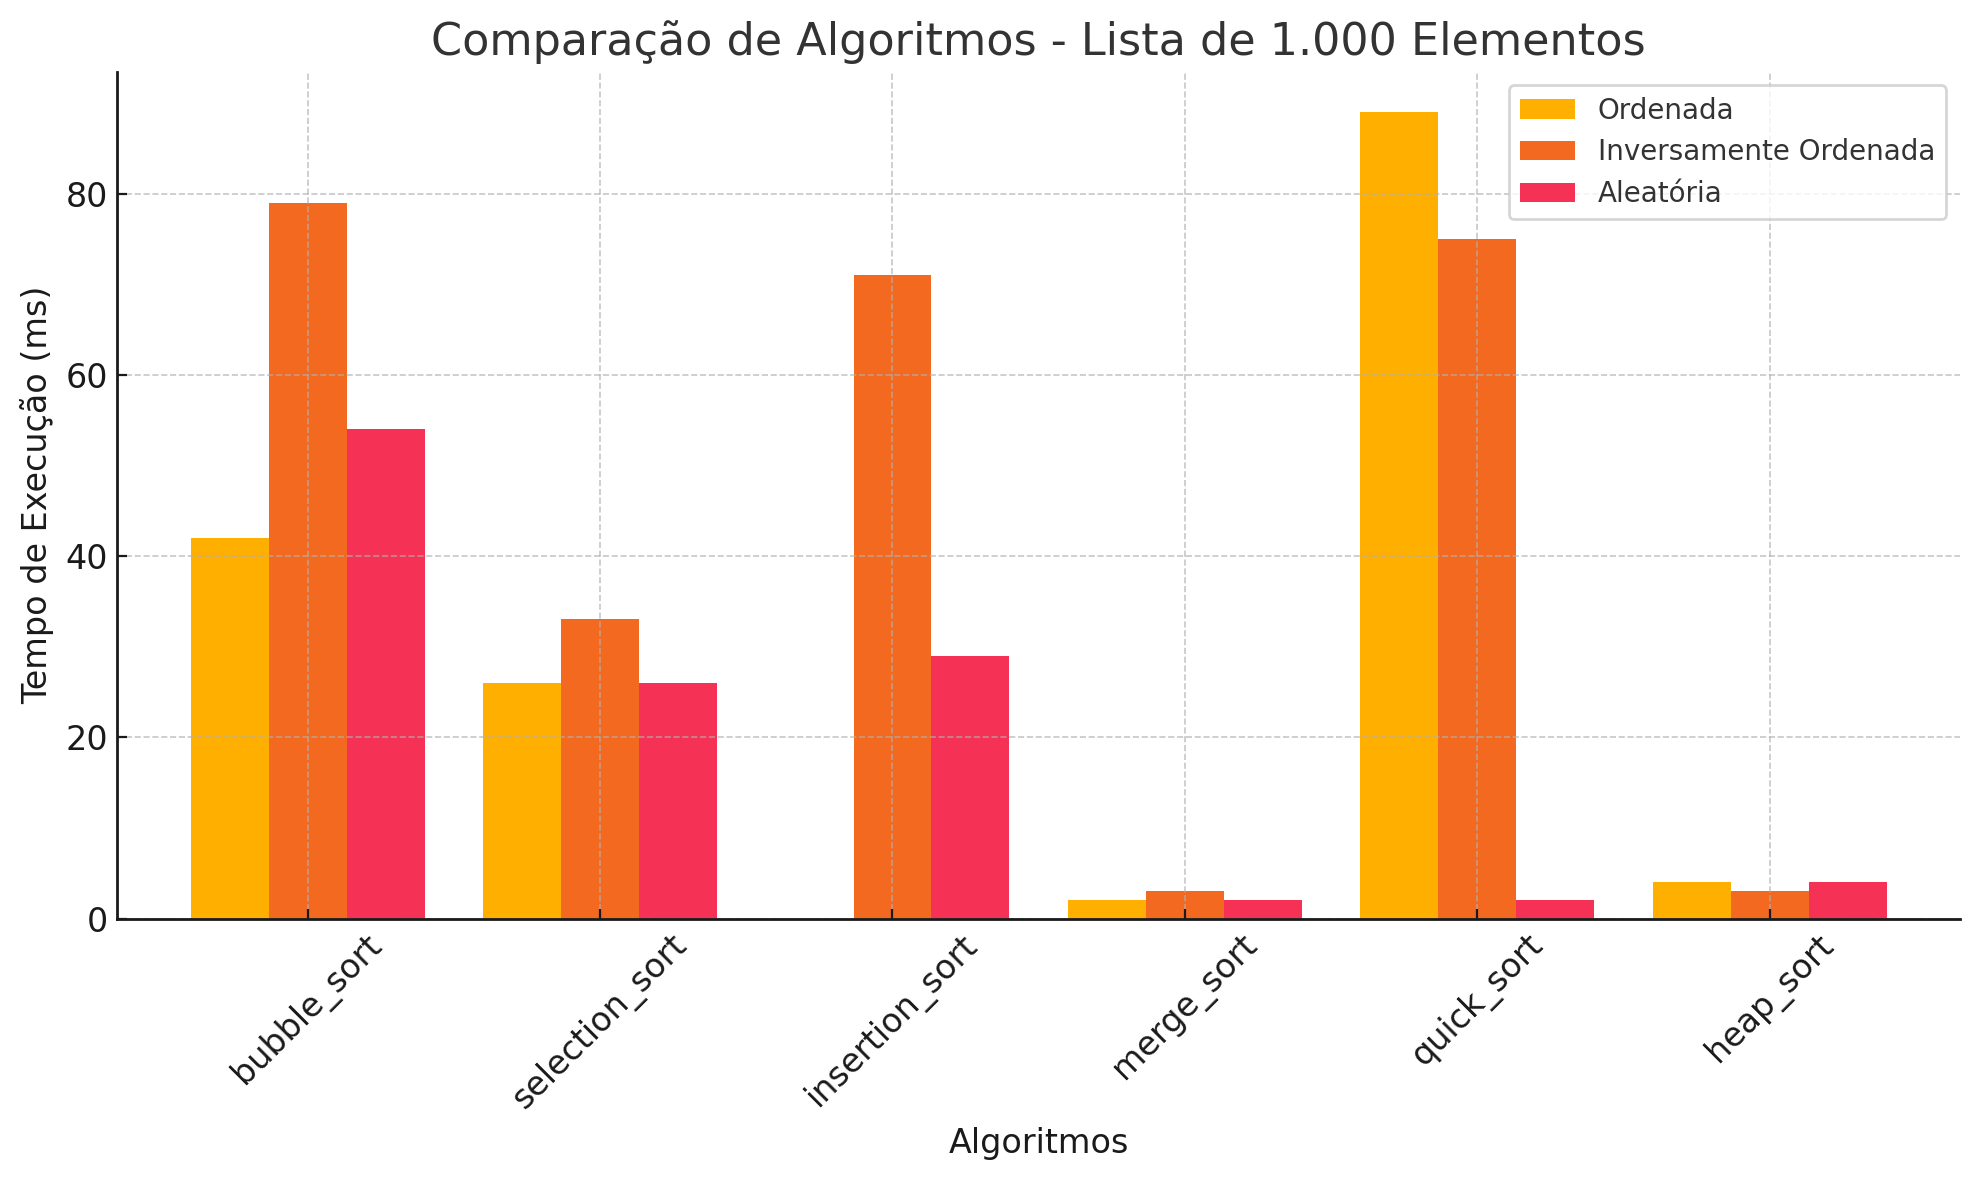
\includegraphics[width=0.8\linewidth]{trabalho/1.000 elementos.png}
    \caption{Gráfico da execução na lista de 1.000 elementos}
    \label{fig:enter-label}
\end{figure}

\begin{figure}[!h]
    \centering
    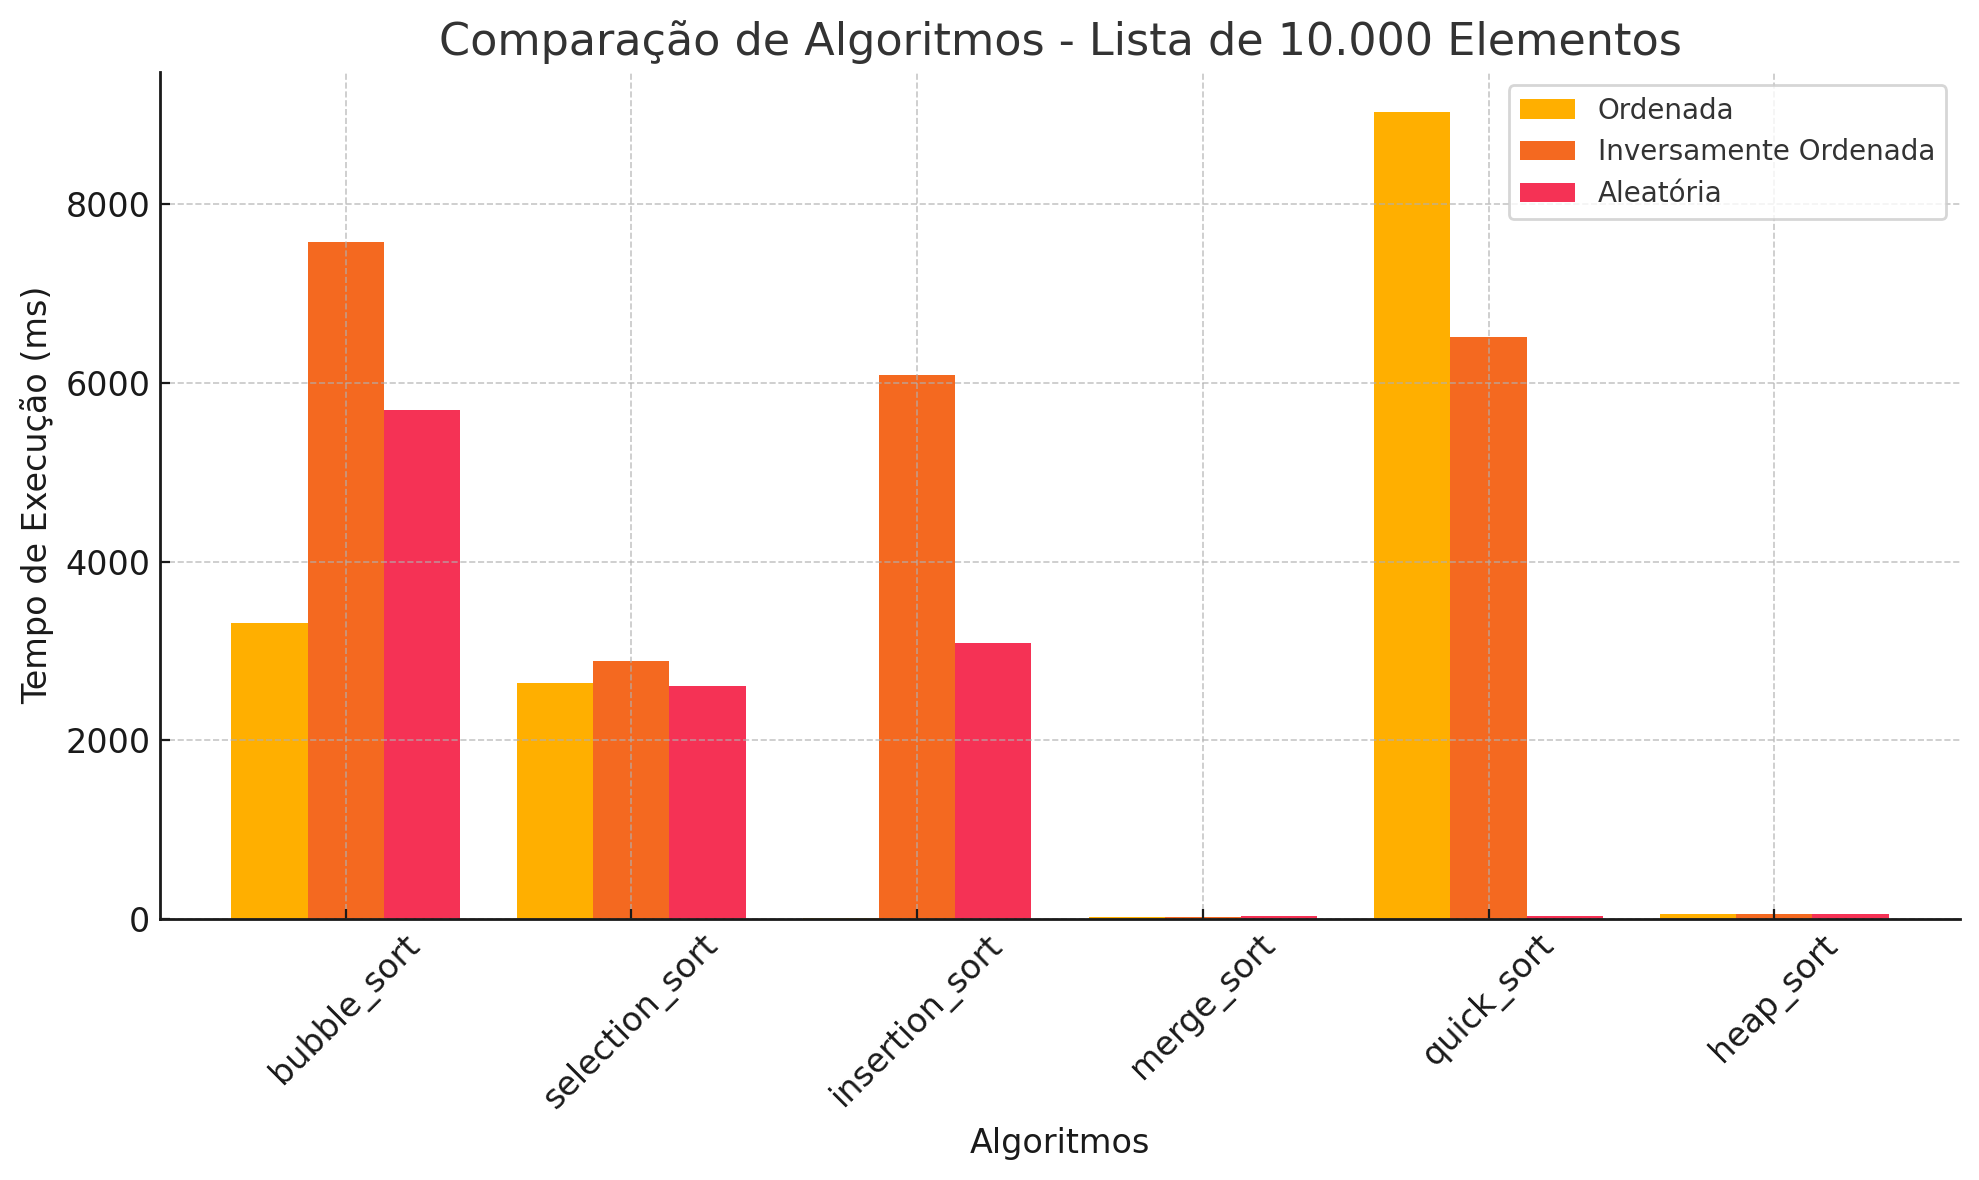
\includegraphics[width=0.8\linewidth]{trabalho/10.000 elementos.png}
    \caption{Gráfico da execução na lista de 10.000 elementos}
    \label{fig:enter-label}
\end{figure}

\begin{figure}[!h]
    \centering
    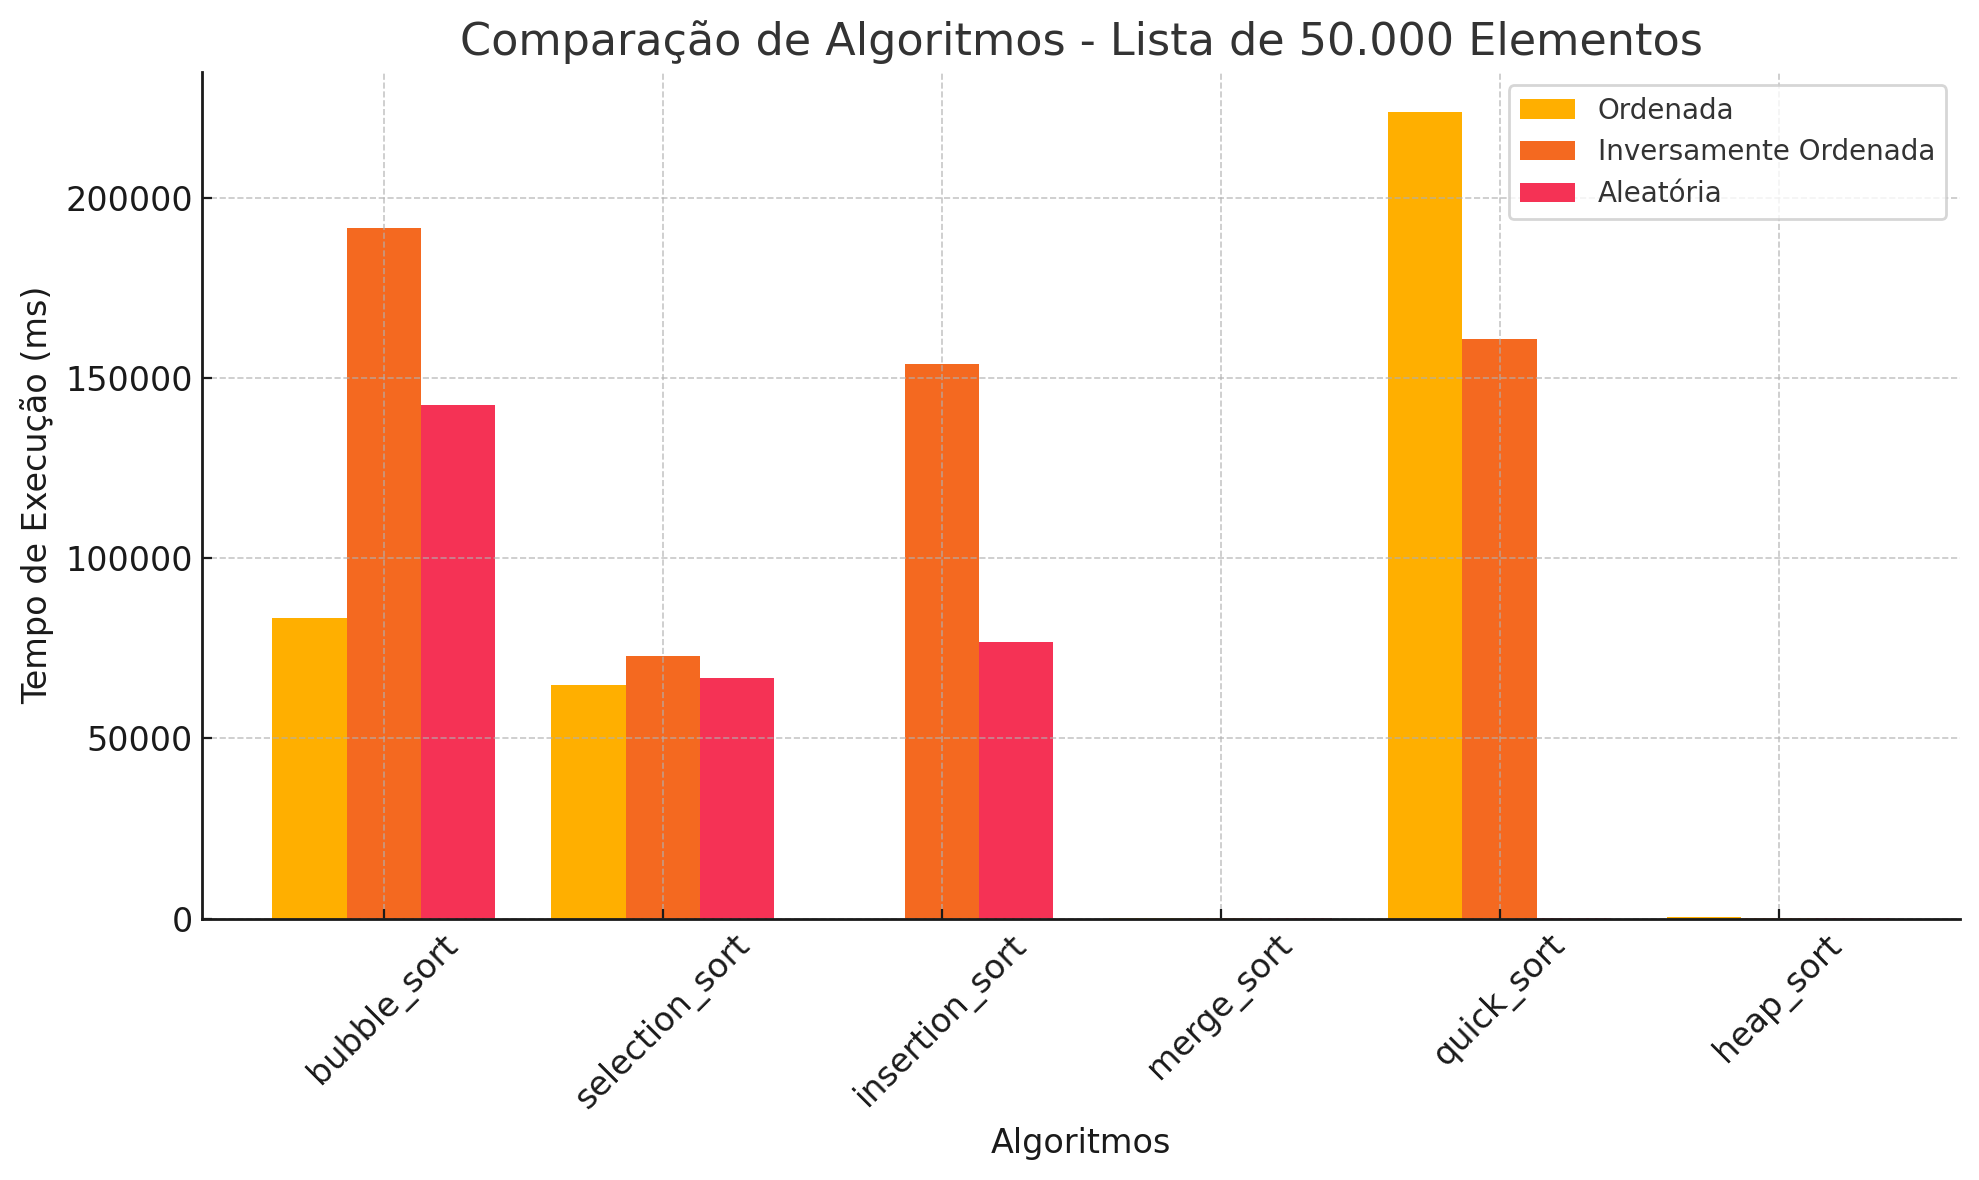
\includegraphics[width=0.8\linewidth]{trabalho/50.000 elementos.png}
    \caption{Gráfico da execução na lista de 50.000 elementos}
    \label{fig:enter-label}
\end{figure}

\begin{figure}[!h]
    \centering
    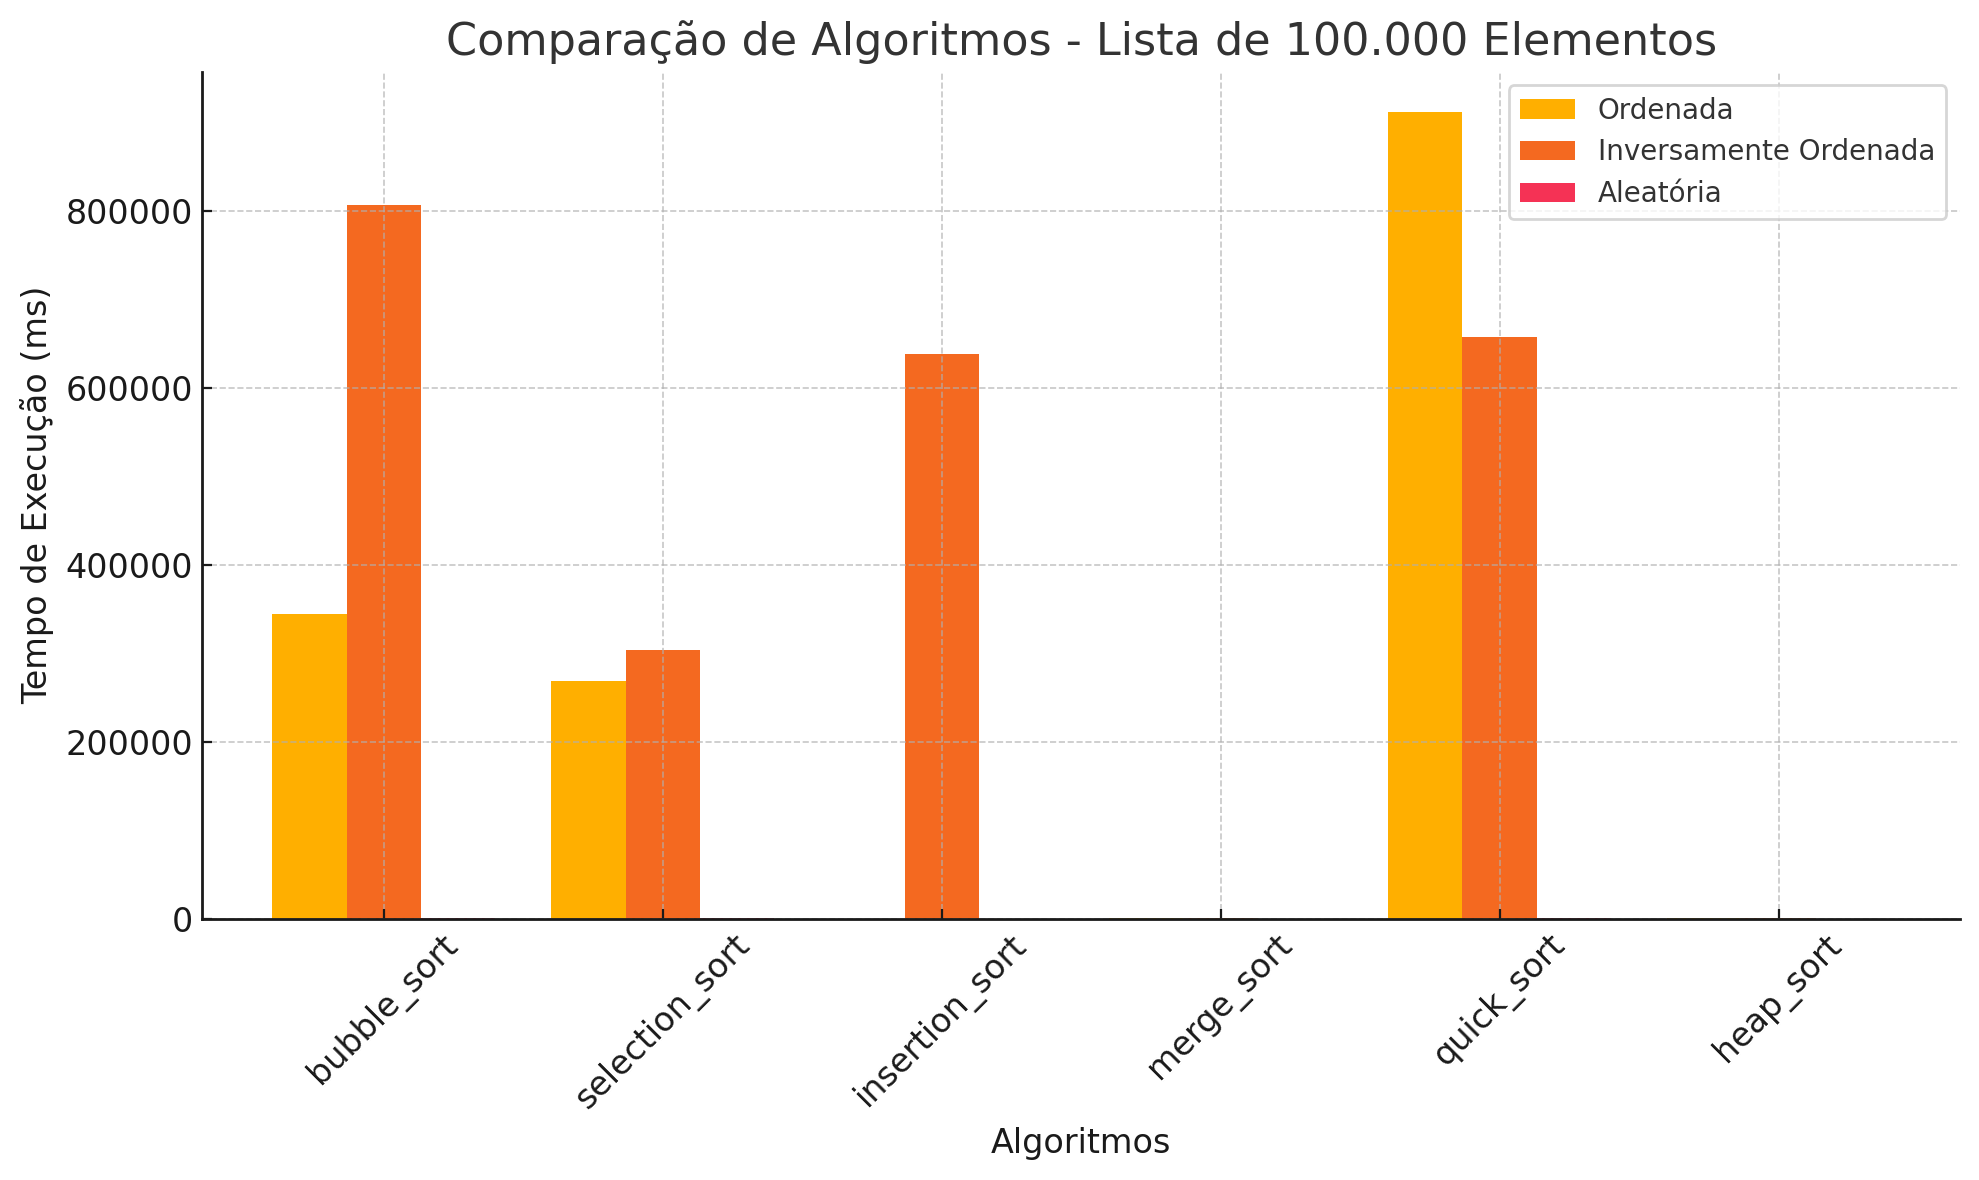
\includegraphics[width=0.8\linewidth]{trabalho/100.000 elementos.png}
    \caption{Gráfico da execução na lista de 100.000 elementos}
    \label{fig:enter-label}
\end{figure}




\chapter{Discussão}
\section{Análise}
A análise dos resultados mostra que a eficiência dos algoritmos de ordenação varia significativamente conforme o tamanho e a organização das listas. De modo geral, os algoritmos com complexidade \(O(n^2)\) (Bubble Sort, Selection Sort e Insertion Sort) apresentaram desempenhos inadequados para listas maiores, especialmente quando estas estavam inversamente ordenadas. Já os algoritmos com complexidade \(O(n \log ⁡n)\) (Merge Sort, Quick Sort e Heap Sort) demonstraram um desempenho superior, com tempos de execução significativamente menores, especialmente para listas aleatórias.

\section{Comparação Teórica}
Conforme esperado, os algoritmos de complexidade quadrática apresentaram desempenho satisfatório apenas em listas pequenas e parcialmente ordenadas, como o Insertion Sort, que teve excelente desempenho em listas previamente ordenadas. No entanto, quando aplicados a listas maiores ou inversamente ordenadas, esses algoritmos apresentaram uma grande quantidade de comparações e trocas, resultando em tempos de execução extremamente elevados.

O Merge Sort, com sua complexidade \(O(n \log ⁡n)\), mostrou ser consistentemente eficiente em todos os cenários. O Quick Sort, embora eficiente para listas aleatórias, apresentou resultados piores em listas ordenadas devido ao número de trocas excessivo. O Heap Sort apresentou desempenho estável em todos os testes, destacando-se como uma alternativa eficiente e de fácil implementação.

\section{Considerações sobre Implementação e Memória}
Em termos de facilidade de implementação, o Bubble Sort, Selection Sort e Insertion Sort são algoritmos simples, mas pouco eficientes em grandes volumes de dados. O Merge Sort requer mais memória por ser um algoritmo de ordenação por divisão e conquista, o que pode ser uma desvantagem em ambientes com restrição de recursos. O Quick Sort, embora eficiente em muitos casos, pode ter um comportamento ineficiente em listas já ordenadas ou inversamente ordenadas.

\section{Limitações do Trabalho e Sugestões Futuros}
O trabalho limitou-se a analisar o tempo de execução, o número de comparações e o número de trocas. Em trabalhos futuros, seria interessante explorar o impacto do uso de memória e realizar análises com outras variações de algoritmos de ordenação, como o Quick Sort com pivôs aleatórios e o Merge Sort in-place. Além disso, investigar o desempenho em diferentes arquiteturas de hardware e ambientes multithread pode ser uma boa sugestão para aprofundar o estudo.

\chapter{Conclusão}
Os resultados deste estudo mostram que algoritmos de complexidade \(O(n^2)\), como o Bubble Sort, Selection Sort e Insertion Sort, são ineficazes para listas grandes, especialmente em cenários onde os dados estão desordenados ou inversamente ordenados. Algoritmos com complexidade \(O(n \log ⁡n)\), como Merge Sort, Quick Sort e Heap Sort, demonstraram um desempenho muito mais eficiente, com destaque para o Merge Sort e Heap Sort em termos de estabilidade e uso de memória. Recomenda-se o uso de algoritmos \(O(n \log⁡ n)\) para listas grandes ou aleatórias, enquanto algoritmos como o Insertion Sort podem ser mais adequados para listas pequenas ou previamente ordenadas.

\backmatter 
\singlespacing   
% ----------------------------------------------------------------------------------------------------- %
\bibliography{trabalho}



\end{document}
